\documentclass[12pt,a4paper]{report}
\let\openright=\cleardoublepage



%%% Choose a language %%%

\newif\ifEN
\ENtrue   % uncomment this for english
%\ENfalse   % uncomment this for czech

%%% Configuration of the title page %%%

\def\ThesisTitleStyle{mff} % MFF style
%\def\ThesisTitleStyle{cuni} % uncomment for old-style with cuni.cz logo
%\def\ThesisTitleStyle{natur} % uncomment for nature faculty logo

\def\UKFaculty{Faculty of Mathematics and Physics}
%\def\UKFaculty{Faculty of Science}

\def\UKName{Charles University in Prague} % this is not used in the "mff" style

% Thesis type names, as used in several places in the title
\def\ThesisTypeTitle{\ifEN BACHELOR THESIS \else BAKALÁŘSKÁ PRÁCE \fi}
%\def\ThesisTypeTitle{\ifEN MASTER THESIS \else DIPLOMOVÁ PRÁCE \fi}
%\def\ThesisTypeTitle{\ifEN RIGOROUS THESIS \else RIGORÓZNÍ PRÁCE \fi}
%\def\ThesisTypeTitle{\ifEN DOCTORAL THESIS \else DISERTAČNÍ PRÁCE \fi}
\def\ThesisGenitive{\ifEN bachelor \else bakalářské \fi}
%\def\ThesisGenitive{\ifEN master \else diplomové \fi}
%\def\ThesisGenitive{\ifEN rigorous \else rigorózní \fi}
%\def\ThesisGenitive{\ifEN doctoral \else disertační \fi}
\def\ThesisAccusative{\ifEN bachelor \else bakalářskou \fi}
%\def\ThesisAccusative{\ifEN master \else diplomovou \fi}
%\def\ThesisAccusative{\ifEN rigorous \else rigorózní \fi}
%\def\ThesisAccusative{\ifEN doctoral \else disertační \fi}



%%% Fill in your details %%%

% (Note: \xxx is a "ToDo label" which makes the unfilled visible. Remove it.)
\def\ThesisTitle{Cross-lingual transfer for the annotation of the SynSemClass ontology}
\def\ThesisAuthor{Petr Kašpárek}
\def\YearSubmitted{2024}

% department assigned to the thesis
\def\Department{Institute of Formal and Applied Linguistics}
% Is it a department (katedra), or an institute (ústav)?
\def\DeptType{Institute}

\def\Supervisor{prof. RNDr. Jan Hajič, Dr.}
\def\SupervisorsDepartment{Institute of Formal and Applied Linguistics}

% Study programme and specialization
\def\StudyProgramme{Computer Science}
\def\StudyBranch{Artificial Intelligence}

\def\Dedication{%
\chapter*{Dedication} I would like to thank my supervisor, prof. RNDr. Jan Hajič, Dr., for suggesting the thesis topic, giving me the opportunity to work on this project and also his help and advice throughout my work on the thesis.

I also would like to thank the consultant of my thesis, RNDr. Jana Straková, Ph.D., for her dedicated help and advice, both on the technical implementation as well as on academic writing. I greatly appreciate the time she spent on giving me advice, detailed explanations of technical problems, as well as the time spent proof-reading the thesis.

I would also like to thank my family.
}

% DEPENDENCY: thesis.xmpdata
\def\AbstractEN{%
This work compares two approaches to automatic preannotation of semantic class to verbs in a sentence for the purpose of adding a new language to the SynSemClass ontology. Both approaches rely on a multilingual deep learning classification model fine-tuned on already annotated English, Czech and German data of the ontology. The first, more classical, approach is annotation projection. It uses a parallel corpus and the aforementioned model to make predictions on a source language already present in the ontology and projects the predictions onto the target language using automated word alignment. The second approach, zero-shot cross-lingual transfer, assumes that the multilingual properties of the underlying model are sufficient and that we can make reasonable predictions directly on the target language, even though the model was never trained for that specific task on the specific target language. For the purpose of evaluation, we manually build and annotate a small Korean language dataset to test the performance on a language significantly different from English, Czech and German. We conclude that the zero-shot approach performs notably better than the alignment approach (p $<$ 0.005) obtaining 0.54 both in recall and precision, compared to 0.37 and 0.41 in recall and precision respectively of the alignment approach. We perform an analysis of the errors and find that the extra steps of annotation projection introduce cascading errors and that loose translation poses a problem in itself.
% ABSTRACT IS NOT A COPY OF YOUR THESIS ASSIGNMENT!
}

\def\AbstractCS{%
Tato práce porovnává dva přístupy k~automatické předanotaci sémantických tříd sloves ve větách za účelem přidání nového jazyka do ontologie SynSemClass. Oba přístupy vycházejí z vícejazyčného deep learning klasifikačního modelu, který byl fine-tunovaný na již anotovaných anglických, českých a~německých datech z ontologie. První, více tradiční, přístup je annotation projection. Používá paralelní korpus a~výše zmíněný model k~vytvoření predikcí na zdrojovém jazyce, který je již obsažen v ontologii, a~tyto predikce projektuje na cílový jazyk pomocí automatického word alignmentu. Druhý přístup, zero-shot cross-lingual transfer, předpokládá, že vícejazykové schopnosti deep learning modelu jsou dostatečné a~že můžeme vytvořit kvalitní predikce přímo na cílovém jazyce, i když model nebyl nikdy trénován pro danou úlohu na daném cílovém jazyce. Pro účely vyhodnocení ručně vytváříme a~anotujeme malý korejský dataset za účelem otestování výsledků na jazyce, který se významně liší od angličtiny, češtiny a~němčiny. Dospíváme k~závěru, že zero-shot transfer vykazuje výrazně lepší výkon než annotation projection (p $<$ 0,005), s hodnotami recall a~precision 0,54, ve srovnání s 0,37 recall a~0,41 precision u~annotation projection. Také provádíme analýzu chyb a~zjišťujeme, že dodatečné kroky annotation projection zavádějí kaskádovité chyby a~že volný překlad sám o~sobě představuje problém.}

% 3 to 5 keywords (recommended), each enclosed in curly braces.
% Keywords are useful for indexing and searching for the theses by topic.
% DEPENDENCY: thesis.xmpdata
\def\Keywords{%
{annotation projection}, {zero-shot cross-lingual transfer}, {ontology}, {multilingual natural language processing}, {lexical semantics}
}

% If your abstracts are long and do not fit in the infopage, you can make the
% fonts a bit smaller by this setting. (Also, you should try to compress your abstract more.)
% Alternatively, consider increasing the size of the page by uncommenting the
% geometry modification in thesis.tex.
\def\InfoPageFont{}
%\def\InfoPageFont{\small}  %uncomment to decrease font size

\ifEN\relax\else
% If you are writing a czech thesis, you additionally need to fill in the
% english translation of the metadata here!
\def\ThesisTitleEN{\xxx{Thesis title in English}}
\def\DepartmentEN{\xxx{Name of the department in English}}
\def\DeptTypeEN{\xxx{Department}}
\def\SupervisorsDepartmentEN{\xxx{Superdepartment}}
\def\StudyProgrammeEN{\xxx{study programme}}
\def\StudyBranchEN{\xxx{study branch}}
\def\KeywordsEN{%
\xxx{{key} {words}}
}
\fi


\usepackage[a-2u]{pdfx}

\ifEN\else\usepackage[czech,shorthands=off]{babel}\fi

% See https://en.wikipedia.org/wiki/Canons_of_page_construction before
% modifying the size of printable area. LaTeX defaults are great.
% If you feel it would help anything, you can enlarge the printable area a bit:
%\usepackage[textwidth=390pt,textheight=630pt]{geometry}
% The official recommendation expands the area quite a bit (looks pretty harsh):
%\usepackage[textwidth=145mm,textheight=247mm]{geometry}

%%% TYPICAL FONT CHOICES (uncomment what you like) %%%
% Recommended combo: Libertinus (autoselects Biolinum for sans) and everything
% else (math+tt) comes from Latin Modern)
\usepackage{lmodern}
\usepackage[mono=false]{libertinus}

% For the "classic" LaTeX fonts (very good for pure math theses), simply
% comment out the libertinus package above.

% IBM Plex font suite: nice, but requires us to fine-tune the sizes and does
% not directly support small caps (\textsc):
%\usepackage[usefilenames,RM={Scale=0.88},SS={Scale=0.88},SScon={Scale=0.88},TT={Scale=0.88},DefaultFeatures={Ligatures=Common}]{plex-otf}

% TeX Gyre combo (Pagella+Heros+Cursor)
%\usepackage{fontspec}
%\setmainfont{TeX Gyre Pagella}
%\setsansfont{TeX Gyre Heros}
%\setmonofont{TeX Gyre Cursor}

% some useful packages
\usepackage{microtype}
\usepackage{amsmath,amsfonts,amsthm,bm}
\usepackage{graphicx}
\usepackage{xcolor}
\usepackage{booktabs}
\usepackage{caption}
\usepackage{floatrow}

\usepackage{kotex}
\usepackage{svg}
\usepackage{wrapfig}
\usepackage{subcaption}

%\usepackage[natbib,style=authoryear,sorting=none,maxcitenames=1,maxnames=1,maxbibnames=6]{biblatex}

\usepackage[backend=bibtex,natbib,style=authoryear,maxcitenames=2, maxbibnames=6, minbibnames=6, dashed=false]{biblatex}

%\usepackage[style=authoryear,sorting=none,maxcitenames=1,maxnames=1,maxbibnames=6]{biblatex}

% Bibliography formatting.
% CHECK THE REQUIREMENTS OF YOUR DEPARTMENT AND FACULTY ON THE CITATION FORMAT!
%
% These are relatively "safe" default options that most people use:
%\usepackage[natbib,style=numeric,sorting=none]{biblatex}
% alternative with alphanumeric citations (more informative than numbers, and
% more common in computer science journals):
%\usepackage[natbib,style=alphabetic]{biblatex}
%
% ALTERNATIVES THAT CONFORM TO ISO690
% ISO690 is not the greatest citation format ever, but may be formally
% required at Charles University, depending on your faculty and department.
%\usepackage[natbib,style=iso-numeric,sorting=none]{biblatex}
%\usepackage[natbib,style=iso-alphabetic]{biblatex}
% You might want to add extra options such as `maxbibnames=6,maxcitenames=2`
% here to further conform to some of the formatting requirements (see below for
% details). Again, consult your faculty rules.
%
% Additional option choices:
%  - add `giveninits=true` to typeset "E. A. Poe" instead of full Edgar Allan
%  - `terseinits=true` additionaly shortens it to nature-like "Poe EA"
%  - add `maxnames=10` to limit (or loosen) the maximum number of authors in
%    bibliography entry before shortening to `et al.` (useful when referring to
%    book collections that may have hundreds of authors)
%  - use `maxcitenames=2` to finetune the amount of authors listed in text-cite
%    commands (\citet). Corresponding option that only affects the bibliography
%    is `maxbibnames=10`.
%  - `sorting=none` causes the bibliography list to be ordered by the order of
%    citation as they appear in the text, which is usually the desired behavior
%    with numeric citations. Additionally you can use a style like
%    `numeric-comp` that compresses the long lists of citations such as
%    [1,2,3,4,5,6,7,8] to simpler [1--8]. This is especially useful if you plan
%    to add tremendous amounts of citations, as usual in life sciences and
%    bioinformatics.
%  - if you don't like the "In:" appearing in the bibliography, use the
%    extended style (`ext-numeric` or `ext-alphabetic`), and add option
%    `articlein=false`.
%
% possibly reverse the names of the authors with the default styles:
%\DeclareNameAlias{default}{family-given}

% load the file with bibliography entries
\addbibresource{refs.bib}

% remove this if you won't use fancy verbatim environments
\usepackage{fancyvrb}

% remove this if you won't typeset TikZ graphics
\usepackage{tikz}
\usetikzlibrary{positioning} %add libraries as needed (shapes, decorations, ...)

% remove this if you won't typeset any pseudocode
\usepackage{algpseudocode}
\usepackage{algorithm}

% remove this if you won't list any source code
\usepackage{listings}


\hypersetup{unicode}
\hypersetup{breaklinks=true}

\usepackage[noabbrev]{cleveref}


% various forms of TODOs (you should remove this before submitting)
\usepackage[textsize=tiny, backgroundcolor=yellow!25, linecolor=black!25]{todonotes}
\newcommand{\xxx}[1]{\textcolor{red!}{#1}}

% Added by JS
\newcommand{\jana}[1]{\textcolor{magenta}{#1}}
 % remove this before compiling the final version




% use this for typesetting a chapter without a number, e.g. intro and outro
\def\chapwithtoc#1{\chapter*{#1}\addcontentsline{toc}{chapter}{#1}}

\makeatletter
\def\@makechapterhead#1{
  {\parindent \z@ \raggedright \normalfont
   \Huge\bfseries \thechapter. #1
   \par\nobreak
   \vskip 20\p@
}}
\def\@makeschapterhead#1{
  {\parindent \z@ \raggedright \normalfont
   \Huge\bfseries #1
   \par\nobreak
   \vskip 20\p@
}}
\makeatother

% If there is a line/figure overflowing into page margin, this will make the
% problem evident by drawing a thick black line at the overflowing spot. You
% should not disable this.
\overfullrule=3mm

% The maximum stretching of a space. Increasing this makes the text a bit more
% sloppy, but may prevent the overflows by moving words to next line.
\emergencystretch=1em

\ifEN
\theoremstyle{plain}
\newtheorem{thm}{Theorem}
\newtheorem{lemma}[thm]{Lemma}
\newtheorem{claim}[thm]{Claim}
\newtheorem{defn}{Definition}
\theoremstyle{remark}
\newtheorem*{cor}{Corollary}
\else
\theoremstyle{plain}
\newtheorem{thm}{Věta}
\newtheorem{lemma}{Lemma}
\newtheorem{claim}{Tvrzení}
\newtheorem{defn}{Definice}
\theoremstyle{remark}
\newtheorem*{cor}{Důsledek}
\fi

\newenvironment{myproof}{
  \par\medskip\noindent
  \textit{\ifEN Proof \else Důkaz \fi}.
}{
\newline
\rightline{$\qedsymbol$}
}

% real/natural numbers
\newcommand{\R}{\mathbb{R}}
\newcommand{\N}{\mathbb{N}}

% asymptotic complexity
\newcommand{\asy}[1]{\mathcal{O}(#1)}

% listings and default lstlisting config (remove if unused)
\DeclareNewFloatType{listing}{}
\floatsetup[listing]{style=ruled}

\DeclareCaptionStyle{thesis}{style=base,font={small,sf},labelfont=bf,labelsep=quad}
\captionsetup{style=thesis}
\captionsetup[algorithm]{style=thesis,singlelinecheck=off}
\captionsetup[listing]{style=thesis,singlelinecheck=off}

% Customization of algorithmic environment (comment style)
\renewcommand{\algorithmiccomment}[1]{\textcolor{black!25}{\dotfill\sffamily\itshape#1}}

% Uncomment for table captions on top. This is sometimes recommended by the
% style guide, and even required for some publication types.
%\floatsetup[table]{capposition=top}
%
% (Opinionated rant:) Captions on top are not "compatible" with the general
% guideline that the tables should be formatted to be quickly visually
% comprehensible and *beautiful* in general (like figures), and that the table
% "head" row (with column names) should alone communicate most of the content
% and interpretation of the table. If you just need to show a long boring list
% of numbers (because you have to), either put some effort into showing the
% data in an attractive figure-table, or move the data to an attachment and
% refer to it, so that the boredom does not impact the main text flow.
%
% You can make the top-captions look much less ugly by aligning the widths of
% the caption and the table, with setting `framefit=yes`, as shown below.  This
% additionally requires some extra markup in your {table} environments; see the
% comments in the example table in `ch2.tex` for details.
%\floatsetup[table]{capposition=top,framefit=yes}

\ifEN\floatname{listing}{Listing}
\else\floatname{listing}{Výpis kódu}\fi
\lstset{ % use this to define styling for any other language
  language=C++,
  tabsize=2,
  showstringspaces=false,
  basicstyle=\footnotesize\tt\color{black!75},
  identifierstyle=\bfseries\color{black},
  commentstyle=\color{green!50!black},
  stringstyle=\color{red!50!black},
  keywordstyle=\color{blue!75!black}}

% Czech versions of the used cleveref references (It's not as convenient as in
% English because of declension, cleveref is limited to sg/pl nominative. Use
% plain \ref to dodge that.)
\ifEN\relax\else
\crefname{chapter}{kapitola}{kapitoly}
\Crefname{chapter}{Kapitola}{Kapitoly}
\crefname{section}{sekce}{sekce}
\Crefname{section}{Sekce}{Sekce}
\crefname{subsection}{sekce}{sekce}
\Crefname{subsection}{Sekce}{Sekce}
\crefname{subsubsection}{sekce}{sekce}
\Crefname{subsubsection}{Sekce}{Sekce}
\crefname{figure}{obrázek}{obrázky}
\Crefname{figure}{Obrázek}{Obrázky}
\crefname{table}{tabulka}{tabulky}
\Crefname{table}{Tabulka}{Tabulky}
\crefname{listing}{výpis}{výpisy}
\Crefname{listing}{Výpis}{Výpisy}
\floatname{algorithm}{Algoritmus}
\crefname{algorithm}{algoritmus}{algoritmy}
\Crefname{algorithm}{Algoritmus}{Algoritmy}
\newcommand{\crefpairconjunction}{ a~}
\newcommand{\crefrangeconjunction}{ a~}
\fi

% My commands
\newcommand{\ort}[1]{\textlangle\nobreak#1\nobreak\textrangle}
\newcommand{\ortx}[2]{\textit{#2} \textlangle\nobreak#1\nobreak\textrangle}
 % use this file for various custom definitions


\begin{document}

% the layout is mandatory, edit only in dire circumstances

\pagestyle{empty}
\hypersetup{pageanchor=false}
\begin{center}

% top part of the layout, this actually differs between faculties

\def\ThesisTitleXmff{%
  \ifEN
    \centerline{\mbox{\includegraphics[width=166mm]{img/logo-en.pdf}}}
  \else
    \centerline{\mbox{\includegraphics[width=166mm]{img/logo-cs.pdf}}}
  \fi
  \vspace{-8mm}\vfill%
  {\bf\Large\ThesisTypeTitle}
  \vfill%
  {\LARGE\ThesisAuthor}\par
  \vspace{15mm}%
  {\LARGE\bfseries\ThesisTitle}
  \vfill%
  \Department}
\def\ThesisTitleCuniLogo#1{%
  {\large\UKName\par\medskip\par\UKFaculty }
  \vfill%
  {\bf\Large\ThesisTypeTitle}
  \vfill%
  \includegraphics[width=70mm]{#1}
  \vfill%
  {\LARGE\ThesisAuthor}\par
  \vspace{15mm}%
  {\LARGE\bfseries\ThesisTitle}
  \vfill%
  \Department\par}
\def\ThesisTitleXcuni{\ThesisTitleCuniLogo{img/uklogo.pdf}}
\def\ThesisTitleXnatur{\ThesisTitleCuniLogo{img/naturlogo.pdf}}

% choose the correct page and print it
\csname ThesisTitleX\ThesisTitleStyle\endcsname
% latex corner: X is the new @

\vfill

{
\centerline{\vbox{\halign{\hbox to 0.45\hsize{\hfil #}&\hskip 0.5em\parbox[t]{0.45\hsize}{\raggedright #}\cr
\ifEN Supervisor of the \ThesisGenitive thesis:
\else Vedoucí \ThesisGenitive práce: \fi
& \Supervisor \cr
\noalign{\vspace{2mm}}
Consultant of the \ThesisGenitive thesis:
& RNDr. Jana Straková, Ph.D. \cr
\noalign{\vspace{2mm}}
\ifEN Study programme: \else Studijní program: \fi
& \StudyProgramme \cr
\noalign{\vspace{2mm}}
\ifEN Study branch: \else Studijní obor: \fi
& \StudyBranch \cr
}}}}

\vfill

\ifEN Prague \else Praha \fi
\YearSubmitted

\end{center}

\newpage

% remember to sign this!
\openright
\hypersetup{pageanchor=true}
\pagestyle{plain}
\pagenumbering{roman}
\vglue 0pt plus 1fill

\ifEN
\noindent
I declare that I carried out this \ThesisAccusative thesis independently, and only with the cited
sources, literature and other professional sources. It has not been used to obtain another
or the same degree.
\else
\noindent
Prohlašuji, že jsem tuto \ThesisAccusative práci vypracoval(a) samostatně a výhradně
s~použitím citovaných pramenů, literatury a dalších odborných zdrojů.
Tato práce nebyla využita k získání jiného nebo stejného titulu.
\fi

\ifEN
\medskip\noindent
I understand that my work relates to the rights and obligations under the Act No.~121/2000 Sb.,
the Copyright Act, as amended, in particular the fact that the Charles
University has the right to conclude a license agreement on the use of this
work as a school work pursuant to Section 60 subsection 1 of the Copyright~Act.
\else
\medskip\noindent
Beru na~vědomí, že se na moji práci vztahují práva a povinnosti vyplývající
ze zákona č. 121/2000 Sb., autorského zákona v~platném znění, zejména skutečnost,
že Univerzita Karlova má právo na~uzavření licenční smlouvy o~užití této
práce jako školního díla podle §60 odst. 1 autorského zákona.
\fi

\vspace{10mm}


\ifEN
\hbox{\hbox to 0.5\hsize{%
In \hbox to 6em{\dotfill} date \hbox to 6em{\dotfill}
\hss}\hbox to 0.5\hsize{\dotfill\quad}}
\smallskip
\hbox{\hbox to 0.5\hsize{}\hbox to 0.5\hsize{\hfil Author's signature\hfil}}
\else
\hbox{\hbox to 0.5\hsize{%
V \hbox to 6em{\dotfill} dne \hbox to 6em{\dotfill}
\hss}\hbox to 0.5\hsize{\dotfill\quad}}
\smallskip
\hbox{\hbox to 0.5\hsize{}\hbox to 0.5\hsize{\hfil Podpis autora\hfil}}
\fi

\vspace{20mm}
\newpage

% dedication

\openright

\noindent
\Dedication

\newpage

% mandatory information page

\openright

\vbox to 0.49\vsize{\InfoPageFont
\setlength\parindent{0mm}
\setlength\parskip{5mm}

\ifEN Title: \else Název práce: \fi
\ThesisTitle

\ifEN Author: \else Autor: \fi
\ThesisAuthor

\DeptType:
\Department

\ifEN Supervisor: \else Vedoucí \ThesisGenitive práce: \fi
\Supervisor, \SupervisorsDepartment

Consultant:
RNDr. Jana Straková, Ph.D., \SupervisorsDepartment

\ifEN Abstract: \AbstractEN \else Abstrakt: \AbstractCS \fi

\ifEN Keywords: \else Klíčová slova: \fi
\Keywords

\vss}\ifEN\relax\else\nobreak\vbox to 0.49\vsize{\InfoPageFont
\setlength\parindent{0mm}
\setlength\parskip{5mm}

Title:
\ThesisTitleEN

Author:
\ThesisAuthor

\DeptTypeEN:
\DepartmentEN

Supervisor:
\Supervisor, \SupervisorsDepartmentEN

Abstract:
\AbstractEN

Keywords:
\KeywordsEN

\vss}
\fi

\newpage

\openright
\pagestyle{plain}
\pagenumbering{arabic}
\setcounter{page}{1}


\tableofcontents


\chapwithtoc{Introduction}

Semantic ontologies are important linguistic resources that capture our knowledge of the world. Such lexical resources provide a solid foundation for theoretical linguistic research and become building blocks for other natural language processing research. We work with the multilingual ontology SynSemClass \parencite{uresova-etal-2020-synsemclass} that catalogues semantic classes of word senses. Currently, it only contains verbs.

Manually annotating such ontology is costly. Previously, the SynSemClass project utilized existing lexical resources to build up and extend the ontology. However, rich lexical resources are rare and not harmonized into the same format and a common annotation guideline, thus their usage cannot be easily streamlined. We want to be able to easily extend the ontology for a new language without these resources. In order to do this, we implement a toolchain that creates automatic annotation suggestions. These suggestions will be then given to human annotators who will review them and integrate the correct suggestions into the ontology and discard the erroneous suggestions.

To this end, we use existing tools and evaluate two methods of using these tools. Both of these methods rely on a deep learning classification model for SynSemClass \parencite{SSC_LLM_Suggestions}. The first method, annotation projection, utilizes a sentence-aligned parallel corpus. The method consists of generating annotations on a source language natively supported by the classification model and projecting those automatic annotations onto the target language using automatic word alignment. The second method, zero-shot cross-lingual transfer, relies on the multilingual pretraining of the classification model and generates predictions directly on the target text.

To evaluate the performance of these two methods, we chose Korean as our target language. Korean is an agglutinative head-final East Asian language. This sets it apart from the European head-initial languages that are currently part of the SynSemClass ontology, namely English, Czech, German and Spanish. We build a small Korean--English parallel corpus and manually annotate it for semantic classes and word alignment. We then measure the performance for both methods and verify that the difference is statistically significant.

After discovering that zero-shot cross-lingual transfer performs significantly better, we dive deeper into the reasons why. We find that the loose non-verbatim translation poses a fundamental limit to annotation projection. The text is often rephrased such that the verbs we want to project often change meaning or are eliminated entirely. Furthermore, we show that errors in word alignment contribute to the overall error. We conclude the classification model performs roughly the same on both Korean and English under ideal conditions, but the extra steps of annotation projection introduce cascading errors. 

The last step is creating the final annotation suggestions. Since the classification model creates predictions on single mentions of verbs, our goal is to aggregate the individual predictions into a single suggestion for each class-lemma pair. In \cref{sec:aggregation_experiment}, we investigate what the most efficient aggregation strategy is.

\chapter{Background}


\section{SynSemClass}

The SynSemClass lexicon \parencite{uresova-etal-2020-synsemclass} --- formerly CzEngClass --- is a multilingual event-type ontology currently under development. An event-type ontology is a hierarchy of classes that denote events and states. Each class is populated by class members --- words. Unrelated to our work, the SynSemClass project also seeks to link the classes and its members to a plethora of existing lexical resources, such as the EngVallex \parencite{EngVallex20}, CzeEngVallex \parencite{czengvallex}, FrameNet \parencite{ruppenhofer2016framenet}, PropBank \parencite{kingsbury2002treebank} and many others. The lexicon currently consists of words from English, Czech, German and Spanish. See \cref{fig:synsemclass-scheme} for the scheme of the lexicon and \cref{fig:synsemclass-tools} for the tools used to view the ontology data. The goal of this bachelor thesis is to explore machine learning methods as preprocessing steps to automatically suggest annotations for extending the ontology into a new language.

\begin{figure}[h]
\centering
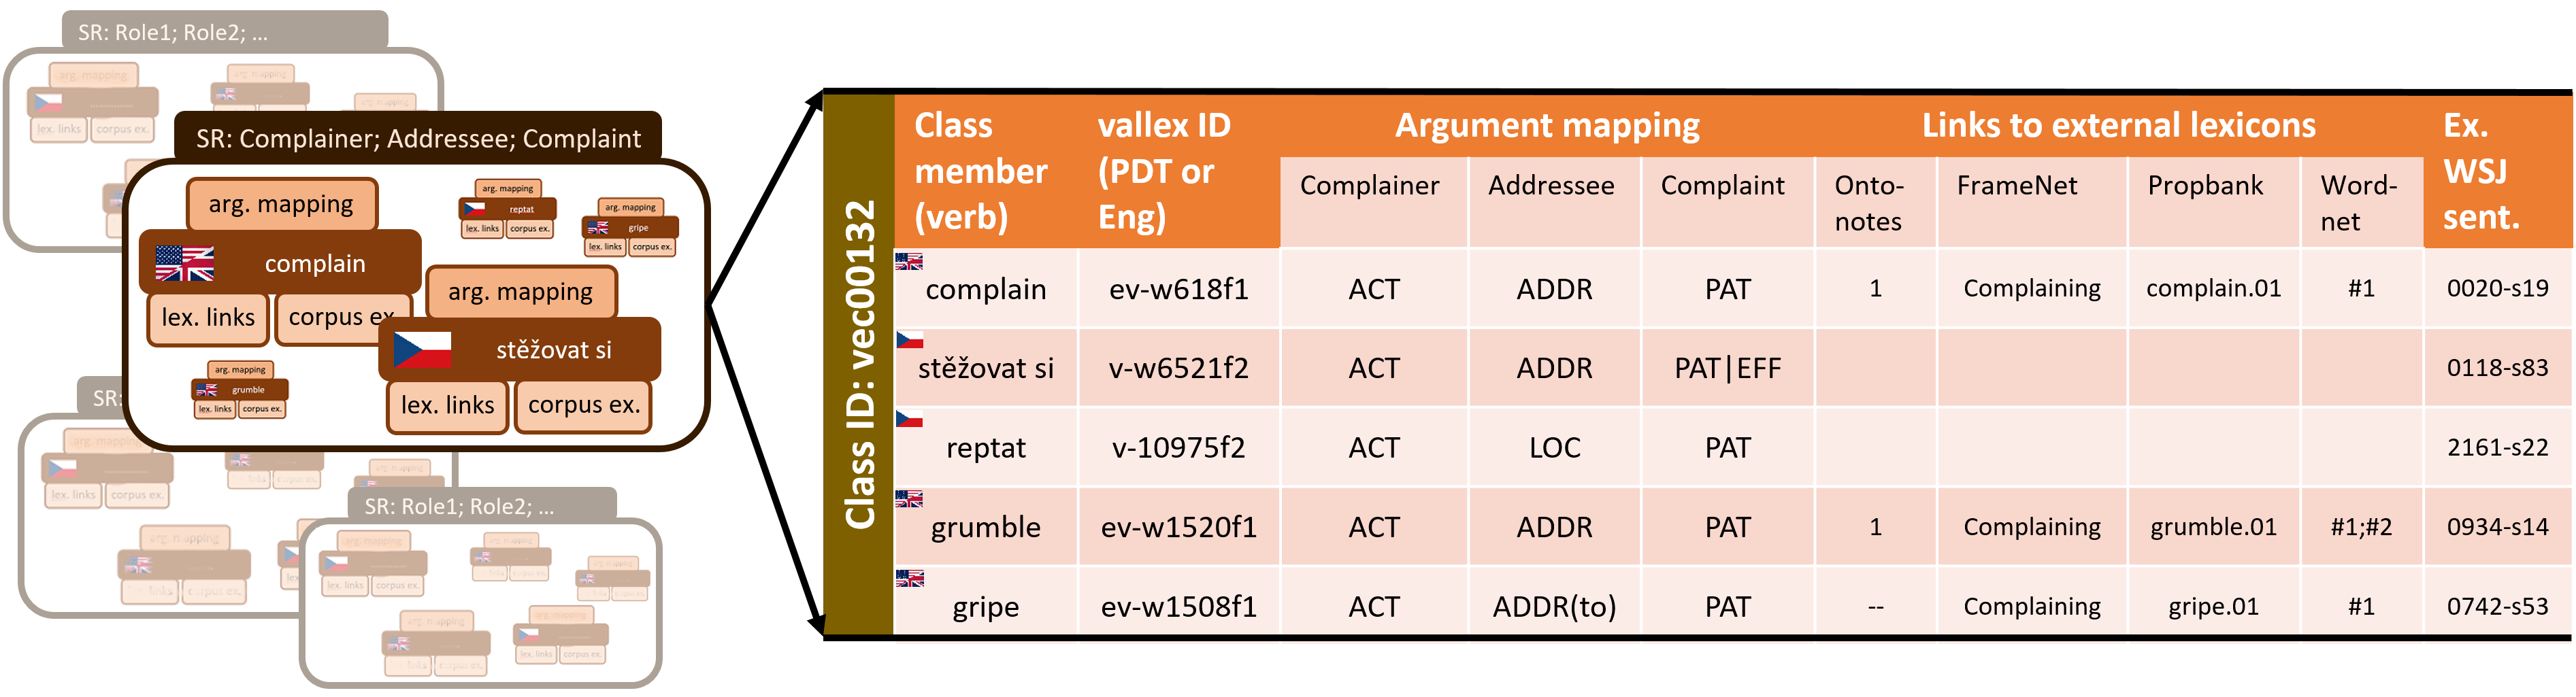
\includegraphics[width=0.9\linewidth]{img/06-final-ssclass-scheme}
\caption{The overall scheme of the SynSemClass lexicon and an example of a class (“complain-stežovat si”) \parencite{uresova-etal-2020-synsemclass}.}
\label{fig:synsemclass-scheme}
\end{figure}

In the rest of this section, we briefly summarize the initial annotation process of the ontology. We focus only on the steps that are relevant to us and omit the rest.

\citet{ssc_start} built the first Czech and English version of the lexicon by semi-randomly choosing Czech verbs of various frequencies from the Prague Czech-English Dependency Treebank (PCEDT) \parencite{pcedt} and letting those be the names and seeds of new classes. They used automatic word alignment to get the English counterparts. Manual pruning and annotation followed. The PCEDT corpus contains an annotation layer relating to semantics and deep syntax, the so called tectogrammatical layer. \citet{ssc_start} used this information to build the links to other resources as well as other linguistic annotation, which we will not delve into, as it does not affect our work. 

German was added by \citet{uresova-etal-2022-making} by automatically word-aligning the English-German part of the ParaCrawl \parencite{banon-etal-2020-paracrawl} corpus. They decided on a set of English verbs, for which they found the most common German alignments. These were then manually filtered and annotated for correct classes. As they did not use a part-of-speech tagger, they could not distinguish between verb and noun forms of the verb (e.g., `to run' vs. `a run') and these cases had to be manually removed.

\begin{figure}[t]
\centering
\begin{subfigure}[t]{0.49\textwidth}
\centering
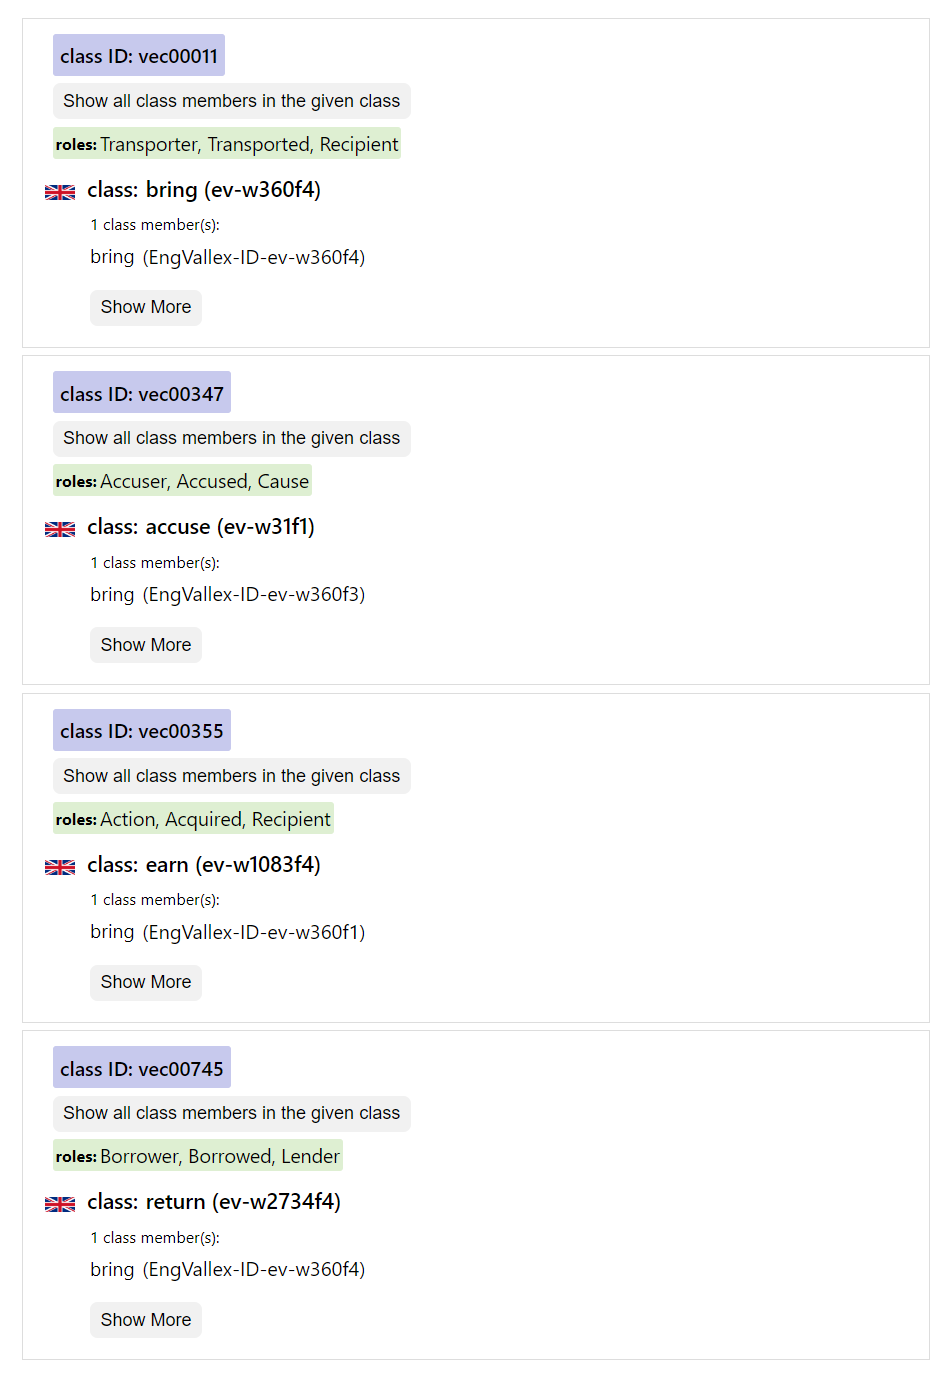
\includegraphics[width=0.9\linewidth]{img/synsemclass_tool}
\caption{A lookup of the word `bring' in the SynSemClass Search\footnotemark tool shows that it belongs into multiple classes.}
\label{fig:synsemclass-search}
\end{subfigure}\hfill
\begin{subfigure}[t]{0.49\textwidth}
\centering
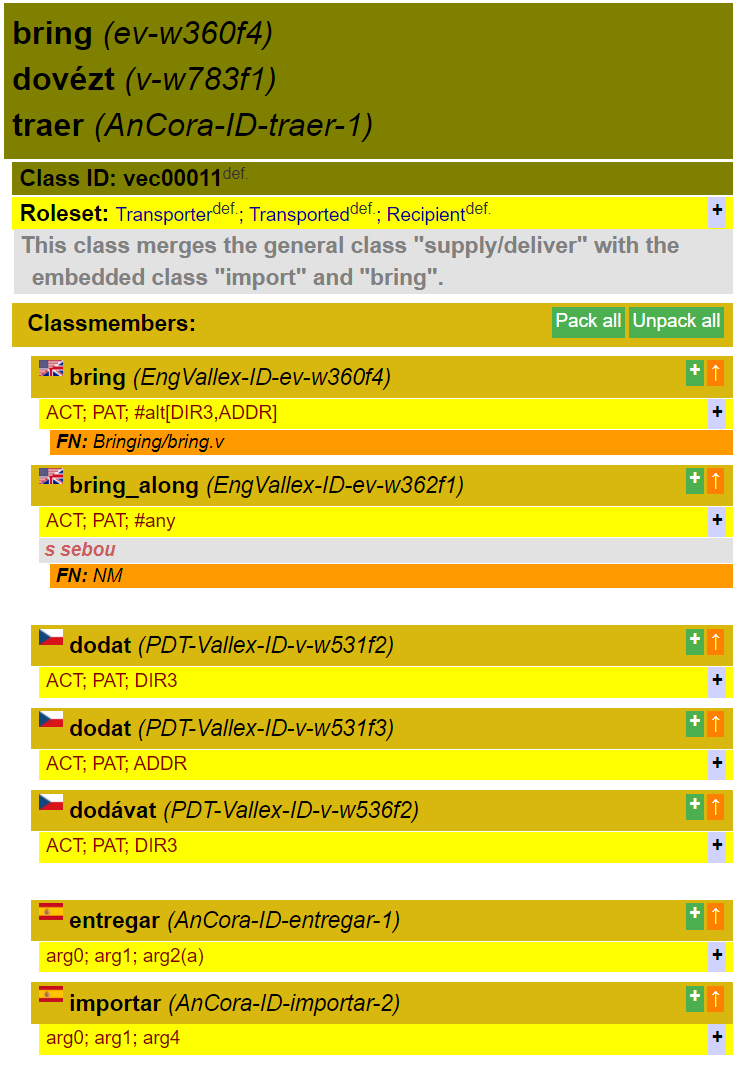
\includegraphics[width=0.9\linewidth]{img/synsemclass_class}
\caption{The class with ID vec00011 has several words associated with it as shown in the browse tool.\footnotemark}
\label{fig:synsemclass-browse}
\end{subfigure}
\caption{Two different tools for the SynSemClass ontology. Note that both results are trimmed.}
\label{fig:synsemclass-tools}
\end{figure}

\addtocounter{footnote}{-1}
\footnotetext{\url{https://lindat.mff.cuni.cz/services/SynSemClassSearch/}}
\addtocounter{footnote}{1}
\footnotetext{\url{https://lindat.cz/services/SynSemClass50/SynSemClass50.html}}

The Spanish part \parencite{SSC_Spanish} was built in a similar manner to German, using automatic word alignment on parallel data. Additionally, they used semantic information extracted from a Spanish lexical resource, AnCora \parencite{taule-etal-2008-ancora}, to perform automatic filtering. Although AnCora contains only Spanish lemmas, it links to several English resources that are also linked in the SynSemClass ontology. If the automatic alignment created alignments for which semantic data was linkable to AnCora but the senses did not match, the pairing was discarded. Unlike the German team, they had data tagged for part of speech.

There is a key difference between the initial phases of the SynSemClass annotation and the challenge of a new language presented here. In the initial phases of the SynSemClass annotation, more extensively annotated resources were available, including (automatically) word-aligned parallel corpora and manually annotated verb senses with respective valency dictionaries. In our case, the starting point is simply a sentence-aligned parallel corpus between a newly added language and a source language already annotated in the corpus, without any additional semantic information or a valency lexicon in the target language. Our language of choice is Korean. We describe Korean as well as our motivation behind choosing it in the next section.

We note that this work was done on SynSemClass 4.0\footnote{\url{https://lindat.mff.cuni.cz/repository/xmlui/handle/11234/1-4746}}. The current version of SynSemClass is 5.0\footnote{\url{https://lindat.mff.cuni.cz/repository/xmlui/handle/11234/1-5230}}.


\section{Korean language}

We chose Korean as the language on which we test our methods for adding a completely new language into the ontology, as well as the overall design of the ontology to accommodate a non-European language. The author has a lower-intermediate knowledge of Korean, however, we would like to acknowledge that the work has not been checked by anyone either fluent in the language or with a sufficient linguistic background in it. We are confident that any errors made are of low significance and not damaging to the work as a whole. What follows is a brief introduction to the Korean language and its grammar.

Korean is an East Asian language spoken by more than 75 million people, most of whom live on the Korean peninsula. While being similar to Japanese in many aspects, the languages are generally regarded as not related and Korean is attributed its own language family, the Koreanic language family, whose only other member is the Jeju language, spoken by about 5,000 speakers on the island Jeju south of the Korean peninsula. Efforts trying to link Korean and Japanese are complicated by previous use of writing systems based on the Chinese writing system, which can obscure historic pronunciation. In 1443, Korean king Sejong the Great invented and later published a new, more phonemic, script. However, due to resistance from scholars and the upper classes, the script became widely adopted only in the second half of the 20th century.

Nowadays, the Korean script is called Hangul \ort{한글} (with a different name used in North Korea). Depending on the way one counts, it uses 24-51 letters (complex letters are considered to be made of basic letters, however they may have vastly different pronunciation, e.g., ㅏ /a/ + ㅣ /i/ = ㅐ /e/). The letters have mnemonic shapes, see \cref{fig:korean-k} for an example.


\begin{wrapfigure}{r}{0.3\textwidth}
\includesvg[width=0.9\linewidth]{img/korean_k.svg}
\caption{The Korean letter \ort{ㄱ} /k/ is based on the placement of the tongue on the velum. \mbox{Image} adapted from \citet{velar-plossive}.}
\label{fig:korean-k}
\end{wrapfigure}

Similar letters have similar shapes unlike most of the Latin alphabet (e.g., compare the Latin pair \ort{g} \ort{k} and the very roughly equivalent pair in Hangul \ort{ㄱ} \ort{ㅋ}). Hangul letters are arranged into blocks, which consist of three positions for letters --- initial, medial and an optional final position. For example, the letters ㅎ /h/ + ㅏ /a/ + ㄴ /n/ can form the block 한 /han/. For the rest of the work, we will use the Revised romanization system as reference, while also providing the Hangul counterpart.

Korean is an agglutinative language. Agglutination is the process of adding (often multiple) morphemes to a stem of a word, with the stem mostly remaining unchanged. To demonstrate the essence of this process and its difference from inflection, we will try to give an extreme example. It is not typical for a word to have this many morphemes, but it is not rare. \vspace{0.8em}

\begin{tabular}{llll}
성공 & seong-gong  &  & success \\
적 & jeog &  & “ful”, affix meaning of having such character \\
이 & i &  & be \\
었 & eoss &  & past tense \\
다고 & dago &  & quotation \\
\addlinespace
말했다 & malhaessda & & said \\
\addlinespace
\addlinespace
\multicolumn{4}{l}{성공적이었다고 말했다.} \\
\multicolumn{4}{l}{seong-gongjeogieossdago malhaessda.} \\
\multicolumn{4}{l}{`(He) said (he) was successful.'} \\
\end{tabular}
\vspace{0.8em}

In the above example, both subjects are omitted. Without context, it is unclear who said it and who was successful. This phenomenon is called pro drop (pronoun dropping). On top of dropping the subjects as is done in Slavic languages, Korean also allows for dropping of objects thanks to a phenomenon known as topic drop. The common phrase for `I love you.' \ortx{사랑해}{saranghae} does not say who loves whom. An example conversation would be: \vspace{0.8em}

\begin{tabular}{llll}
이 & i  &  & this \\
케이크 & ke-ikeu  &  & cake \\
좋아 & joh-a  &  & good \\
\addlinespace
누가 & nuga  &  & who \\
만들었어 & mandeur-eoss-eo  &  & made \\
\addlinespace
\addlinespace
\multicolumn{4}{l}{이 케이크 좋아. 누가 만들었어?} \\
\multicolumn{4}{l}{i keikeu joh-a. nuga mandeur-eoss-eo?} \\
\multicolumn{4}{l}{`This cake is good. Who made (it)?'} \\
\end{tabular}
\vspace{0.8em}

In Korean, the Subject-Object-Verb (SOV) word order is used, as opposed to English, Czech, German and most European languages, which usually use the Subject-Verb-Object (SVO) word order. This means that typically in a sentence, the subject comes first, followed by the object and the verb being the very last in the sentence.\vspace{0.8em}

\begin{tabular}{llll}
나는 & naneun  &  & I \\
사람 & saram  &  & person \\
만났다 & mannassda &  & met \\
\addlinespace
\addlinespace
\multicolumn{4}{l}{나는 사람 만났다.} \\
\multicolumn{4}{l}{naneun saram mannassda.} \\
\multicolumn{4}{l}{`I met a person.'} \\
\end{tabular}
\vspace{0.8em}

The change in word order is also present elsewhere, most notably in relative clauses, which come before the word they are modifying.\vspace{0.8em}

\begin{tabular}{llll}
바나나 & banana & & banana \\
준 & jun & & gave \\
그 & geu & & that  \\
사람 & saram & & person \\
만났다 & mannassda &  & met \\
\addlinespace
\addlinespace
\multicolumn{4}{l}{바나나 준 그 사람 만났다.} \\
\multicolumn{4}{l}{banana jun geu saram mannassda.} \\
\multicolumn{4}{l}{`(I) met that person who gave (me) a banana.'} \\
\end{tabular}
\vspace{0.8em}

We hope this section was sufficient in giving a very basic overview of the Korean language and its distinction from European languages. We will provide more examples of Korean grammar as they become relevant for the following sections.


\section{Related work}

The task of predicting a SynSemClass ontology class might seem to be the same as word sense disambiguation, but we note that the two tasks are different. \citet{word_sense_disambiguation} defines word sense disambiguation as selecting a single or more senses from a set of possible senses \textit{for the given word}, that is, each word has a different set of possible senses. With the SynSemClass ontology, each verb can be assigned to any of the circa 1000 SynSemClass classes. We cannot limit the scope of the senses simply based on the lemma. That is for several reasons.

Most importantly, the SynSemClass project allows for idiomatic meaning. For example, the expression `to lay the blame on someone' would be annotated the same as `to blame' / `to accuse' \parencite[section 4.3]{uresova-etal-2022-making}. Even if this were not the case, we assume the ontology is still under construction, so the full scope of a word's meaning is not known, either because the given language is only partially annotated, or because we are in the beginning of the process of adding the language to the ontology.

In the case of designing a completely new hierarchy of classes or (word) senses on a given set of words from scratch, unsupervised clusterization techniques have also been suggested, e.g., Brown clustering \parencite{brown-etal-1992-class}. However, our situation differs from such a setting. The ontology is already partially constructed, containing about 1000 classes, and the classes are partially populated with Czech, English, German and Spanish words that express the concepts of those classes. Our challenge is to incorporate words that possibly express the same concept(s) from an incoming new language into one or more of the existing classes or decide that no such class is relevant for the new word.


\chapter{Methodology}
\label{chap:methodology}

Our goal is to help the annotators of the SynSemClass ontology in adding a new language. We merely assume a parallel corpus, as opposed to the lexical resources and semantically annotated corpora available for the previously incorporated languages. To this end, we rely on a machine-learning classification model by \citet{SSC_LLM_Suggestions}. For a given sentence, this model is able to predict the SynSemClass class for a marked verb. In this context, we evaluate two methods, both using this model, for adding a new language to the ontology. We describe these two methods later in this chapter. Using this model, we produce a preannotated language file. This file contains the verbs and their example usages collected from the corpus, grouped into SynSemClass classes. The task of the human annotators is then to manually accept or decline the automatically generated suggestions.

In this chapter, we describe the Korean data we use for our experiments and the methods we use to extract the annotation suggestions out of them. The details of our Python implementation are described in \cref{implementation} and the user documentation is in \cref{user_doc}.\footnote{Source code: \url{https://github.com/petrkasp/synsemclass-pipeline}}

\section{Source data --- parallel corpora}
\label{sec:data}

After careful consideration we chose to work with data\footnote{\url{https://github.com/jungyeul/korean-parallel-corpora/tree/master/korean-english-news-v1}}  from \citet{park-etal-2016-korean}, in particular their news corpus. The data consists of about 97k sentences. It was crawled from Yahoo! Korea and Joins.com\footnote{The authors list the website as Joins CNN. According to Wikipedia, Joins.com is a (now defunct) website for the newspaper JoongAng Ilbo. We found no information about a link with CNN.} during 2010-2011. The authors provide no further information on the corpus, so the rest is just our observation. The data seem to be pieces of news articles from about 2000 to 2011. There are about 8~sentences per article and the sentences are ordered sequentially, that is in the order as they appeared in the text. Although no explicit article delimiters are included, the articles seem to be ordered chronologically, from the oldest to the newest. We believe the Korean text is original and the English translation is based on it. Sometimes, when English is translated into Korean, the Korean text can suffer from unusual syntactic structures and unnatural word choices. This phenomenon is known as translationese. Fortunately, in this corpus, both the Korean and English texts are of high quality. The sentence alignment is likely done automatically and there are many errors, both complete misalignments and ends or beginnings being cut off. Despite these shortcomings, we judged the corpus to be of the best quality among the parallel corpora available at the time.

We also considered several corpora\footnote{\url{https://opus.nlpl.eu/results/en&ko/corpus-result-table}} from OPUS \parencite{opus}. Although the corpora are much bigger in size, they lack in quality. If we had needed a bigger corpus, our top choice would have been CCMatrix, both in terms of quality and its quantity of 19.4M sentences. The most common problem we see with the OPUS corpora are untranslated sentences aligned with each other. For example, this happens when a quote is left untranslated in the Korean text. Most of the texts also suffer from unnatural translation, although it is possible that this would have not been a problem for us given our focus on verbs.

\section{UDPipe 2 --- finding verbs}

While it is possible that the ontology will expand to different word classes, so far, only verbs are considered. For finding the verbs in the data, we use UDPipe 2 \parencite{straka-2018-udpipe}\footnote{\url{https://github.com/ufal/udpipe/tree/udpipe-2}}. UDPipe 2 is a trainable natural language processing (NLP) pipeline capable of sentence segmentation, tokenization, part-of-speech tagging, lemmatization and dependency parsing. It is trained on the data from Universal Dependencies (UD; \cite{nivre2016universal}). Universal Dependencies is a project that collects treebanks, i.e., corpora annotated for syntactic structure, and provides a unified annotation style and harmonized tagsets for morphological analysis annotation and dependency parsing. It currently contains treebanks for 147 languages. UDPipe 2 provides models for 71 of those languages. The rest of the languages only have small treebanks that are insufficient for training a model.

UDPipe 2 takes in raw text and produces the requested annotations in the CoNNL-U format, which is the format used by Universal Dependencies. We use UDPipe 2 through the LINDAT UDPipe REST Service\footnote{\url{https://lindat.mff.cuni.cz/services/udpipe/}}. For further processing, we consider all words that are tagged \texttt{VERB}, with the exception of words that contain the `to be' \ortx{이}{i} morpheme or end with a common adjective suffix \ortx{스럽다}{seureobda}. We believe that words with this suffix are sometimes incorrectly tagged as verbs due to errors in the UD Korean treebanks. 

\section{Getting Korean lemmas}

We also use UDPipe 2 for finding the lemmas of the verbs. We use the lemmas to group the occurrences to better understand what the correct SynSemClass classes of the lemma are. Unluckily to us, the Korean UD treebanks contain morphological analysis in the lemma field. To get the lemma of a verb, we take the first one or two morphemes and attach the \ortx{다}{da} suffix, which is the suffix of Korean lemmas for verbs and adjectives (sometimes called the dictionary form). If the second morpheme is \ortx{하}{ha} `to do', \ortx{되}{doe} `to become' or \ortx{시키}{shiki} `to order', we replace it with \ortx{하}{ha} `to do' and attach the lemma suffix \ortx{다}{da}. Otherwise, we attach the \ortx{다}{da} suffix directly to the first morpheme.

To explain, Korean verbs can be divided into two groups, ``native" verbs and \ortx{하다}{hada} verbs. The same holds for adjectives as they behave very similarly in terms of syntax. The ``native" verbs form a closed class, new members are rarely added, albeit the class is very large compared to typical closed classes like prepositions. The stem of a ``native" verb is a single morpheme, so we can attach the lemma suffix \ortx{다}{da} directly. Some examples of ``native'' verbs are \ortx{가다}{gada} `to go', \ortx{만들다}{mandeulda} `to make' or \ortx{기다리다}{gidarida} `to wait'.

The \ortx{하다}{hada} verbs are an open class. When a foreign word is borrowed or a new concept needs to be named, a new verb enters the language as a \ortx{하다}{hada} verb. The class is not limited to borrowings and also contains native words (we use the term ``native'' for the other class because of a lack of a better term). \ortx{하다}{hada} verbs are formed by a noun followed by the \ortx{하다}{hada} suffix (where \ortx{다}{da} is the lemma suffix). While \ortx{하다}{hada} is a word on its own with the meaning of `to do', the meaning of the verbs it creates is hardly ``to do something'' in the English sense, e.g., \ortx{말하다}{malhada} `to speak, lit. speech+do', \ortx{행복하다}{haengboghada} `to be happy, lit. happiness+do' (adjective).

The noun part and the \ortx{하다}{hada} part can often be separated, as seen on the example below.\vspace{0.8em}

\begin{tabular}{llll}
준비+를 & junbi+reul  &  & preparation+accusative \\
안 & an  &  & not \\
했어 & haess-eo  &  & didn't do (past tense of \ortx{하다}{hada}) \\
\addlinespace
\multicolumn{4}{l}{준비를 안 했어.} \\
\multicolumn{4}{l}{junbireul an haesseo.} \\
\multicolumn{4}{l}{(I) did not prepare.} \\
\end{tabular}
\vspace{0.8em}

However, not all words are separable, e.g., \ortx{행복하다}{haengboghada}.

The \ortx{하다}{hada} part can be replaced with other suffixes. \ortx{되다}{doeda} `to become' changes the word from active to passive voice and \ortx{시키다}{shikida} `to order' makes the meaning of `make someone do something'. We normalize these to `\ortx{하다}{hada}' to get more precise results. However, some nuance, and perhaps in some cases a wholly different meaning, can be lost.

We note that our lemmatization is not perfect and there are most likely exceptions that break it. Throughout our experiments, we tried to account for everything that came up, but we likely did not cover everything possible.


\section{SimAlign --- making word alignments}
\label{section:simalign}

For annotation projection, word alignments are required. We construct these with SimAlign\footnote{\url{https://github.com/cisnlp/simalign}} \parencite{jalili-sabet-etal-2020-simalign}. SimAlign is a word alignment algorithm based on word embeddings (vector representations of words). It does not require any parallel data for training, only a model that generates the embeddings. This is done with a multilingual large language model (LLM). Embeddings are generated for both sentences, and then words with the closest embeddings are matched. For the matching, the authors propose several algorithms. In their experiments, their novel algorithm IterMax came out on top, so we use this algorithm for the matching. For the language model, we chose XLM-RoBERTa base \parencite{xlmr}. 

At the time of development, we believed SimAlign to be the state of the art, but improvements since have been made in the field \parencite{lai-etal-2022-cross, dou2021word}. In \cref{subs:word_align}, we conduct an experiment where we annotate the word alignment manually and discuss how a potential improvement in word alignment might influence the results.

\section{Predicting SynSemClass classes}

\subsection{SynSemClass classification model}
\label{sec:ssc_pred}

The SynSemClass classification model\footnote{\url{https://github.com/strakova/synsemclass_ml}} \parencite{SSC_LLM_Suggestions} is a classifier
that predicts the SynSemClass class for a marked verb in the input sentence. The verb has to be marked with a caret (\textasciicircum) to determine what verb should be predicted if multiple verbs are in the sentence. (For example, the word `marked' in the following sentence has a mark, ``\mbox{we \textasciicircum{ }marked} the verb in this sentence.'') While \citet{SSC_LLM_Suggestions} only describe working with the Czech part of the ontology, they kindly provided us with a model that was fine-tuned on English, Czech and German data. The extra data for fine-tuning improve performance, reaching 88.83\% accuracy on the Czech test set, compared to 79.17\% accuracy for the model fine-tuned solely on Czech. The combined accuracy on all test data is 86.02\%, with 82.25\% on English and 90.91\% on German.

The foundation for the classification model is the pretrained large language model RemBERT \parencite{chung2021rethinking}. RemBERT is a multilingual masked language model trained on text from Wikipedia and Common Crawl. The RemBERT training data spans 110 languages.\footnote{The full list is available here\\ \url{https://github.com/google-research/google-research/tree/master/rembert}} Masked language modeling is an idea first introduced by \citet{devlin2018bert}. A masked language model (MLM) is trained by masking several random tokens within the text and having the model predict the masked tokens. Unlike classical n-gram language models and generative LLMs, e.g., GPT-style models, the training procedure provides MLMs with the ability to make predictions based on right context. This makes it a good candidate for fine-tuning as classifiers.

When modeling a problem with deep learning, many aspects of the problem need to be considered. One of them are the properties of the predicted data. Usually for classification, the assumption is that there is exactly one correct prediction (e.g., for digit classification, the input image contains exactly one digit 0--9). However, as the SynSemClass ontology is still in development, not all of the classes have been assigned yet. This means that some words do not belong to any class yet. One occurrence of a verb can also belong to multiple classes, if the meaning is not clear. Moreover, we want the model to help us identify suboptimal class definitions. Assume the model is often unsure between two specific classes. This might mean that the two classes are too similar and need merging. For these reasons, \citet{SSC_LLM_Suggestions} modeled the problem as circa 1000 separate binary classifications --- one for each class. This leads to an overwhelming number of negative examples for each classifier (most classes have only a few examples, and even the numerous classes make up only a small portion of the data). Thus during training, instead of using the standard cross entropy loss (an error function used during training) a modification called focal loss \parencite{lin-focal-loss} was used. According to the authors of focal loss, ``focal loss focuses training on a sparse set of hard examples and prevents the vast number of easy negatives from overwhelming the detector during training.''

\subsection{Annotation projection}

Cross-lingual annotation projection is a method that allows us to use a monolingual model to make automatic annotations for different languages other than the natively supported by the model. It relies on having parallel data with word alignments. The word alignments can be manual or they can be automatically generated. We described how we make automatic word alignments in the previous section \ref{section:simalign}.

When working with annotation projection, we talk about two languages. The language supported by the classification model is called the \textit{source} language. We want to create annotations for another language that we call the \textit{target} language. Our source language is English and the target language is Korean. The monolingual model creates annotations in the parallel corpus on the source language text. Then the aligned words in the target language text are assumed to have the same annotation. This process can be quite noisy, due to both noise in the alignment and the classification model.

\subsection{Zero-shot cross-lingual transfer}

In our work, we assume no annotated data for our target language of Korean. However, as the classification model is based on a multilingual large language model, we can try to run it directly on the target language texts. This problem setup is called zero-shot cross-lingual transfer. In this setup, the model is faced with a task that it has not seen during training, but is expected to give reasonable predictions by generalizing the information obtained during pretraining and fine-tuning. See \cref{table:ssc_model} for the zero-shot accuracy of the models provided to us by \citet{SSC_LLM_Suggestions}. 

\begin{table}
\centering
\begin{tabular}{ccc} 
  & All data & Zero-shot \\
 \hline
 English & 82.25\% & 63.59\% (--18.66\%) \\ 
 Czech & 88.83\% & 73.58\% (--15.25\%) \\
 German & 90.91\% & 44.44\% (--46.47\%) \\
\end{tabular}
\caption{Accuracy of the SynSemClass classification models on the three languages available in the ontology. The results in the All data column are based on a single model fine-tuned on all three languages. The results in the Zero-shot column are each for a different model. These models saw no examples of the test language during fine-tuning and were fine-tuned only on the other two languages.}
\label{table:ssc_model}
\end{table}

\section{Evaluation data}
\label{sec:eval_data}

To evaluate the two approaches described in the previous section, we need gold data. In order to be able to do this evaluation on Korean, we built a small corpus manually annotated for SynSemClass classes. Unlike the gold data for Czech, English and German extracted from the existing lexicon, we annotate every single verb in the sentences. This complete annotation alleviates some problems with the aggregation experiments we describe in \cref{sec:aggregation_experiment}.

We start with the news corpus described in \cref{sec:data} and use both annotation projection and zero-shot cross-lingual transfer to give us suggestions for the classes. We then go and remove misaligned sentences (15 in total), add verbs missed by the system, fix incorrect word alignment and select correct SynSemClass classes for each of the verbs, all manually by hand. In order to give the best chances to annotation projection, we also denote how accurate our manual alignment is. In many cases, no good alignment is possible. This happens because the translation is not literal. For example, in one of the sentences, the phrase \ortx{실바가 이끄는 당의 붉은 깃발}{shilbaga ikkeuneun dang-ui bulg-eun gisbal} `the red flag of the party led by Silva' is translated as `his [Silva's] party's red flag'.

In this manner, we manually annotate 131 verbs in 39 sentences. Selecting the correct SynSemClass class out of the total of 884 semantic classes was a very difficult and time consuming task, especially since the SynSemClass search tool was not available at the time.

The format of the pregenerated suggestions and finished annotated parallel corpus is described in \cref{parallel_corpus_format}.

\chapter{Experiments \& results}

In this chapter we describe the experiments we conducted with the toolchain composed of the tools introduced in the previous chapter. We also present the results of the experiments and undertake an analysis of the source of the errors made by the toolchain.

In our main experiment, we determine whether annotation projection or zero-shot cross-lingual transfer performs better on our task of creating suggestions for a semantic ontology. We also give statistical significance for this finding. After concluding that zero-shot cross-lingual transfer performs better, we explore the shortcomings of annotation projection. We find that a fundamental limitation lies in the translation itself and that it often has a meaning too different to be useful for determining the semantic class on the other language side.

In our second experiment, we determine the best parameters for our toolchain with the zero-shot cross-lingual transfer approach. Specifically, we explore what the best way to aggregate the predictions is. 

\section{Is annotation projection or zero-shot transfer better?}
\label{sec:exp1}

We explore and compare the performance of annotation projection and zero-shot cross-lingual transfer. We conduct this experiment on the individual predictions, not on the aggregates. This allows us to explore the reasons behind the errors and better understand them.

\subsection{Metrics}
\label{subsec:metrics}
Our focus is on two metrics --- recall and precision. The two metrics are widely used across computer science, and even in other fields (perhaps under different names). As there is some nuance in their usage, we dive into their definitions a little deeper.

Recall is fundamentally defined as the ratio of correct predictions and the maximum number of correct predictions achievable. Precision is the ratio of correct predictions and the total number of predictions. In classification (into two classes, one of them being the positive class), recall and precision are defined as follows:
\begin{equation*}
\begin{split}
\text{recall} & = \frac{\text{true positives}}{\text{true positives} + \text{false negatives} } \\[1em]
\text{precision} & = \frac{\text{true positives}}{\text{true positives} + \text{false positives}}
\end{split}
\end{equation*}
In information retrieval, recall is the ratio of the retrieved documents that are relevant and the total number of relevant documents, while precision is defined as the ratio of the retrieved documents that are relevant and the total number of retrieved documents.

Our system has characteristics of both. While we indeed classify words into semantic classes, we need to find them in the text first. Even after we find the verb, annotation projection can in some sense reject to classify the verb if there is nothing aligned with it. Thus for a verb to be a correct prediction, three things need to happen:

\begin{enumerate}
    \itemsep0em
    \item UDPipe 2 has to correctly classify it as a verb.
    \item SimAlign needs to align it.
    \item The SynSemClass classification model needs to classify it into the correct class.
\end{enumerate}

Step 2 is not needed with zero-shot cross-lingual transfer and we later show that this is a substantial advantage.

Thus for our purposes, we define recall as the ratio of correct predictions as described above and the total number of gold verbs. Precision is the ratio of correct predictions and the number of verbs found by UDPipe 2, with annotation projection, they also need to be aligned.

\subsection{Zero-shot cross-lingual transfer wins as a system}

We now measure the performance of the two methods when composed into the whole system. In \cref{subs:components}, we measure the performance of each individual component.

Our system consists of taking the raw sentences in the corpus (i.e., without the verb marks) and having UDPipe find the verbs in the Korean text. With zero-shot cross-lingual transfer, we predict the SynSemClass classes directly on the discovered Korean verbs. With annotation projection, we first use SimAlign to find the counterparts on the English side and make the predictions on the aligned English words. Here, many adjustments that could improve the precision of the alignments are possible, e.g., filtering the alignments for part-of-speech, finding the verbs on the English side and doing the alignments vice-verse, or somehow crosschecking these two approaches. To account for these possible changes, in \cref{subs:word_align}, we conduct an oracle experiment where we use manual gold word alignments.

The results are presented in \cref{table:system_results}. On our data, zero-shot transfer significantly outperforms annotation projection in both metrics. As the amount of data we have is rather small, we also perform a statistical test. We chose to do a permutation test on sentences with Monte Carlo sampling with 10k samples. The results are in \cref{table:system_results}. They indicate that the findings are statistically significant.

\begin{table}
\centering
\begin{tabular}{rcc} 
  & Recall & Precision  \\
 \hline
 Annotation projection & 0.37 &  0.41 \\ 
 Zero-shot transfer &  \textbf{0.54} & \textbf{0.54} \\
 \hline
 p-value & 0.00040 & 0.00110
\end{tabular}
\caption{Performance of the two methods used in the overall system with automatic verb identification and word alignment. The p-value indicates the probability of zero-shot transfer outperforming annotation projection by chance.}
\label{table:system_results}
\end{table}

\subsection{Non-verbatim translation is a fundamental limitation}
\label{subs:word_align}

As we described in \cref{sec:eval_data}, during the manual annotation of alignment in the Korean corpus, we encountered many examples of verbs that did not have a proper counterpart on the English side. Thus we divide the gold manual alignments into three groups. In the \textit{none} group, no alignment is possible due to different phrasing and non-literal translation. The \textit{dubious} alignment group are verbs that had a verb of a wholly different meaning or not a verb at all as their aligned counterpart. The rest of verbs fall into the \textit{good} alignment group.

We perform experiments on the portions of the data that contain only the given quality alignment group or better. For both zero-shot cross-lingual transfer and annotation projection, we remove UDPipe 2 and instead use our annotations directly. For annotation projection, we conduct the experiments both with and without the automatic word aligner. Note that is experiment also assumes perfect sentence alignment throughout. The results of the experiment, as well as how much of the data is covered by each quality requirement, are presented in \cref{table:alignment}. In this experiment, we simply use accuracy and omit recall or precision when they are equivalent to accuracy.

We see that the good alignments make up only 73\% of the data. We consider this to be a significant limitation for the possible quality of annotation projection. The quality of the predictions increases as the quality of the alignment increases. The predictions on our manual alignment outperform the predictions on the automatically aligned words and the performance increases in accordance with our alignment groups. This is in accord with previous literature. \citet{behzad2023effect} recently reported on how manual correction of word alignment quality can improve performance on the downstream task.

The experiment also reveals that the accuracy of the model in the zero-shot setting on Korean is 66\%. Interestingly, it is highest when all data are included and falls when we omit the sentences that had no alignment to English. We hypothesize that common fixed expressions are mostly translated non-verbatim, but we did not investigate this idea further. Annotation projection also achieves 66\% in its ideal setting with ideal word alignments. However, if automatic alignment is used, it again trails behind.  



\begin{table}
\centering
\begin{tabular}{rccc} 
& \multicolumn{3}{c}{Alignment type} \\
 & None & Dubious & Good \\
\hline
\textbf{Coverage}  & 100\% & 83\% & 73\% \\
\hline
\textbf{Zero-shot} \\
Accuracy & \textbf{66\%} & \textbf{62\%} & 62\% \\
\hline
\textbf{Annotation projection} \\
\textit{manual alignments} \\
Accuracy & 51\% & 61\% & \textbf{66\%} \\
\textit{automatic alignments} \\
Accuracy & 46\% & 52\% & 57\% \\
Precision & 55\% & 58\% & 61\% \\
\hline
\textbf{Word alignment} \\
Accuracy & 60\% & 62\% & 66\% \\
Precision & 62\% & 69\% & 71\% \\
Rejection rate & 16\% & 10\% & 6\% 
\end{tabular}
\caption{The quality of predictions and automatic word alignments under each type of alignment. We split the best possible word alignment into three categories introduced in \cref{sec:eval_data}. The coverage row describes how much of the data fits into this category or any better. We perform the experiments on this portion of the data. Where either precision or recall is not specified, its meaning is the same as accuracy. The word alignment section describes only the performance of the word aligner, not any predictions. Rejection rate is the ratio of words that were not aligned with anything.}
\label{table:alignment}
\end{table}

\subsection{Error contribution of each component}
\label{subs:components}

In \cref{table:components}, we summarize the performance of each component. When we reported the results of the whole system in \cref{table:system_results}, the results reflected that the system can reject some input verb early on. This verb does not proceed to the next components, e.g., UDPipe 2 fails to find a specific verb. To truly see the effect of each individual component, we give them the gold results of the previous step as input. For this reason, the product of the performances of each individual component does not equal the performance of the whole system. Every component is penalized for failing on the same hard example, while the system could reject it early on.

\begin{table}[h]
\centering
\begin{tabular}{ll} 
\multicolumn{2}{l}{\textbf{UDPipe 2 --- finding verbs}} \\
\addlinespace
Recall & 75\%\\
Precision & 76\% \\
Extra verbs per sentence & 0.85 \\
\addlinespace
\hline
\addlinespace
\multicolumn{2}{l}{\textbf{Translation}} \\
\addlinespace
Verbs alignable & 73\% \\
\addlinespace
\hline
\addlinespace
 \multicolumn{2}{l}{\textbf{SimAlign --- Word alignment}} \\
 \addlinespace
 Accuracy & 66\% \\
 Precision & 71\% \\
 \addlinespace
 \hline
 \addlinespace
\multicolumn{2}{l}{\textbf{SynSemClass classification model}} \\
\addlinespace
Korean: Accuracy & 66\% \\
English: Accuracy & 66\% \\
\end{tabular}
\caption{Performance of each component in separation. We also include the translation as a ``component'', as we believe it to be a integral part of annotation projection and a likely point of failure. The reported values are independent of each other --- they are measured in ideal conditions for that component (gold outputs of previous steps). Thus, if multiplied, they do not equal the results in \cref{table:system_results}. Here, each component is penalized for failing on the same hard examples the previous components failed on.}
\label{table:components}
\end{table}

As we have seen, the accuracy of annotation projection is hindered by non-verbatim translation. More loose styles of translation are very common for high quality translations such as in our corpus. For this reason, we also think of translation as an inherent component of the annotation projection. Another crucial step we do not take into account is sentence alignment. We only work with examples that are properly aligned on the sentence level. During the annotation of our evaluation data, we discarded all sentences with improper sentence alignment.\footnote{We kept a few pairs where the source English sentence had extra words compared to the Korean target sentence, as this did not prevent word alignment.} Of the 54 sentences considered, we kept 72\% of them, however, some were discarded due to other reasons than bad alignment, e.g., a lack of any verbs.

The results show that, on our data, the classification model performs roughly the same on English and Korean. This might be due to the Korean text being original and the English text being the translation, thus the English translation can be possibly slightly unnatural or perhaps just different than natural English text. We cannot rule out that the results would be different for translation in the opposite direction. However, in our setting, the translation and automatic alignment (both on words and likely on sentences) introduce extra error.

\section{Best aggregation parameters}
\label{sec:aggregation_experiment}

We established that zero-shot cross-lingual transfer performs better than annotation projection. Now our goal is to produce the annotation suggestions for the SynSemClass ontology using the preferred method. We need to make the suggestions as aggregations of the the individual predictions, both for practical and technical reasons. The suggestions need to be of high quality and the optimum trade-off between the number of displayed and still relevant suggestions must be found in order to save the costly time of annotators. Here we try to determine what are the most efficient ways to aggregate the predictions for specific precision/recall requirements by studying the precision-recall curves.

An annotation suggestion is a class-lemma pair and each suggestion appears at most once. This is given by the language-specific SynSemClass file format in which the suggestions are to be stored. The SynSemClass classification model gives us probabilities\footnote{The term probability might not be completely accurate here, as the values do not sum to 1 due to the way the problem is modeled as explained in \cref{sec:ssc_pred}.} how likely each example is to be of the given sense and we need to aggregate them into these suggestions. As we want to evaluate the best aggregation strategy as well as an optimal threshold on the final aggregation score, we need gold data of accepted and rejected suggestions. For this purpose we leverage our existing evaluation data. Alongside our manually annotated Korean--English parallel corpus, we also have the examples extracted from the existing ontology.

Both of these datasets are gold annotated sentences, not samples of rejected and accepted annotation suggestions, but under the right assumptions, we can use them to decide whether an automatic suggestion should be rejected or accepted. We generate the suggestions using the text from the corpus and evaluate them using the following rules:

\begin{enumerate}
    \itemsep0em
    \item If the suggestion contains a lemma that is not annotated in our gold data, the suggestion is ignored, i.e., considered neither correct nor wrong.
    \item The suggestion is accepted if there exists an example in the corpus that supports that suggestion. This means there must be a sentence in the corpus that contains the same lemma with the class the suggestion is proposing.
    \item Otherwise, we reject the suggestion.
\end{enumerate}

We need to apply step 1 because the examples from the ontology contain unannotated verbs. The sentences showcase a single class on a single verb, but a lot of the sentences contain other verbs that are not annotated. Unfortunately, this approach introduces several problems:

\begin{enumerate}
    \itemsep0em
    \item[a)] If the system overgenerates, e.g., incorrectly labels a word as a verb, it is ignored. This can slightly inflate the measured performance.
    \item[b)] A single lemma can have different meanings. Suppose that a lemma is present in the corpus with two meanings, but only one of them is annotated. If the system finds the unannotated verb and makes a suggestion based on it, it is incorrectly punished. This can lower the measured performance.
    \item[c)] A slightly more nuanced version of problem b) --- even if all verbs in the corpus were annotated, we still do not cover every correct suggestion. The system might mislabel a verb with a class that is not correct in the given context, but might be correct in another context. As we also take into account other predictions than the top one, this might introduce some false errors.
\end{enumerate}

Fortunately, problems a) and b) do not apply to our Korean--English corpus, as we have manually labeled every verb. On the other hand, the corpus is very small, so the effect of aggregation is barely observable.

We conduct the experiments and take the described problems into account when interpreting the results. On the Korean dataset, we do not apply the filtering rule (rule 1) as it is not needed as explained above. In all experiments, we generate precision-recall curves and compare the results. For easier comparison, we set the ranges of all figures to a fixed value, so some of the figures have a lot of empty padding. All experiments in this section use zero-shot cross-lingual transfer. To better understand the results, we also provide the the dataset sizes in \cref{table:dataset_size}.

\begin{table}
\centering
\begin{tabular}{lc} 
Language & Sentences \\
\hline
\textbf{Partially annotated} \\
English & 7896 \\ 
Czech & 8942 \\ 
German & 985 \\ 
\hline
\textbf{Fully annotated} \\
Korean & 39 \\ 
\end{tabular}
\caption{Dataset sizes in sentences.}
\label{table:dataset_size}
\end{table}

\subsection{Best aggregation function}

We consider four aggregation functions: average, maximum, summation and a probabilistically motivated function we shortly explain. As their input, the functions take all predictions on a specific lemma and a specific SynSemClass class. On each verb example, we consider all 884 predicted probabilities for each class, not just the top one. With the averaging function, we also conduct further experiments how limiting the tail predictions affects the results. For the maximum aggregation function, this limiting would have little effect due to it deciding only on the largest value for the given lemma-class pair.

The probabilistic function assumes that the suggestion is correct, if at least one prediction is correct, and that the predictions are independent. The function is then defined as:

$$
prob(X) = 1 - \prod_i 1 - prob(X_i)
$$

\Cref{fig:agg_functions} shows the results. The German and Korean datasets do not show much difference between the functions. We believe this is due to their small sizes. Due to this, the effects of aggregation are hardly seen. On English and Czech, we can observe that for high precision (high thresholds, small recall), average is dominating. However, for high recall (small threshold, small precision), maximum wins. We explain this intuitively --- for a high recall, every high probability prediction is worth considering, even though there are a lot of small value predictions for this class-lemma pair.

\begin{figure}[h]
\centering

\begin{subfigure}[t]{0.5\textwidth}
\centering
\includesvg[width=1\linewidth]{img/pr/eng_fnc.svg}
\end{subfigure}%
%
\begin{subfigure}[t]{0.5\textwidth}
\centering
\includesvg[width=1\linewidth]{img/pr/ces_fnc.svg}
\end{subfigure}

\begin{subfigure}[t]{0.5\textwidth}
\centering
\includesvg[width=1\linewidth]{img/pr/deu_fnc.svg}
\end{subfigure}%
%
\begin{subfigure}[t]{0.5\textwidth}
\centering
\includesvg[width=1\linewidth]{img/pr/ko-mini-raw_fnc.svg}
\end{subfigure}

\caption{Precision-recall curves for various aggregation functions.}
\label{fig:agg_functions}
\end{figure}

\subsection{Preaggregation filtering}

In the previous experiment, we considered all 884 values, one for each class, predicted by the classifier on each mention of a verb. This includes a lot of very small values around and below 1\% that influence the results. We test whether it is effective to filter those small values before aggregation. There two ways to do this --- setting a threshold for probability, e.g., ignoring everything below 5\%, or only considering the top $K$ predictions for each lemma. The results for the thresholding approaches are displayed in \cref{fig:agg_thr} and the results for top-$K$ are in \cref{fig:agg_prek}.

\begin{figure}[h]
\centering

\begin{subfigure}[t]{0.5\textwidth}
\centering
\includesvg[width=1\linewidth]{img/pr/eng_thr.svg}
\end{subfigure}%
%
\begin{subfigure}[t]{0.5\textwidth}
\centering
\includesvg[width=1\linewidth]{img/pr/ces_thr.svg}
\end{subfigure}

\begin{subfigure}[t]{0.5\textwidth}
\centering
\includesvg[width=1\linewidth]{img/pr/deu_thr.svg}
\end{subfigure}%
%
\begin{subfigure}[t]{0.5\textwidth}
\centering
\includesvg[width=1\linewidth]{img/pr/ko-mini-raw_thr.svg}
\end{subfigure}

\caption{Precision-recall curves for filtering predictions with a probability threshold. Some curves suddenly end as they do not have a high recall portion. This is because the setting inherently only shows high precision results and completely filters out the unlikely suggestions.}
\label{fig:agg_thr}
\end{figure}



\begin{figure}[h]
\centering

\begin{subfigure}[t]{0.5\textwidth}
\centering
\includesvg[width=1\linewidth]{img/pr/eng_pre_k.svg}
\end{subfigure}%
%
\begin{subfigure}[t]{0.5\textwidth}
\centering
\includesvg[width=1\linewidth]{img/pr/ces_pre_k.svg}
\end{subfigure}

\begin{subfigure}[t]{0.5\textwidth}
\centering
\includesvg[width=1\linewidth]{img/pr/deu_pre_k.svg}
\end{subfigure}%
%
\begin{subfigure}[t]{0.5\textwidth}
\centering
\includesvg[width=1\linewidth]{img/pr/ko-mini-raw_pre_k.svg}
\end{subfigure}

\caption{Precision-recall curves for filtering predictions by taking only the top $K$ values into account for each lemma. Kinf means all values. Same as with \cref{fig:agg_thr}, some curves end abruptly and do not have a high recall portion. This is because the setting inherently only shows high precision results and completely filters out the unlikely suggestions. }
\label{fig:agg_prek}
\end{figure}

We see trends similar to the results for aggregation functions. The curves for German and Korean, as well as the high precision parts of the curves for English and Czech behave the same. The curves suggest that it is better not to limit the input, i.e., no threshold and all predictions, not just top $K$ predictions. We see this as intuitive, if we take more input, we get more precise results and suggestions that are not certain are pushed down. For the high recall parts of the curve, a good threshold seems to be around 3\% and the best $K$, for top $K$ predictions, seems to be 3. At the same time, the maximum aggregation function performs very similarly to these two settings.

\subsection{Possible limitations}

We now consider the effects of the problems described earlier and think of how they affect the results. In a large corpus, we can encounter polysemantic verbs that often appear with two or more senses. It is possible that one of the senses is in our gold data while the others are not, even though they are all correct. As we aggregate a large number of predictions, the scores of these polysemantic verbs are lowered. This can give higher measured precision to the final suggestions, as the other senses of the polysemantic verbs are falsely labeled as errors, but with more predictions, their scores are lowered. This is in agreement with our observation that the aggregation function of average with no filtering performs the best for high precision of the suggestions. However, we see that average with no filtering performs well on Korean, too, and we think that Korean does not suffer from the described problems. The difference between average with no filtering and the other approaches is not as prominent there, but it is still clearly dominating.

As for using maximum or filtering for higher recall, we would expect the opposite with the previous line of reasoning. Moreover, the actual difference might be even larger than we measured and using maximum and filtering might be more beneficial than our results suggest. While we lay some groundwork for the optimal parameters, we believe that it would be best to do the measurements again when the annotation phase starts and more data is available.




%\chapter{Discussion}


\chapwithtoc{Conclusions}

We implemented and optimized a toolchain for creating annotation suggestions for the semantic ontology SynSemClass. Unlike the previous work on the ontology, we did not have access to any lexical or semantic resources. We evaluated two approaches --- annotation projection that uses a parallel corpus to project predicted classes from a source language to the target language, and zero-shot cross-lingual transfer that relies on the ability of a machine learning model to generalize to a language it was not trained on. For the purpose of the experiments, we developed and manually annotated for semantic classes a small Korean--English corpus. We found that zero-shot cross-lingual transfer performs significantly better both in terms of recall and precision and verified this statistically.

In order to generate high-value annotation suggestions that are likely to be accepted by annotators, we compared various aggregation approaches using precision-recall curves. We found that taking the average of all predictions including all predictions for each example and not limited to the top one works well. In scenarios where high recall is desired, it seems beneficial to either use maximum instead of average, or take only the three best predictions, or only consider predictions with probability higher than 3\%.

We also analyzed why zero-shot cross-lingual transfer performs better. We found that non-verbatim translation poses a fundamental problem as sometimes the text is rephrased in such a way that the verb disappears or changes meaning significantly. All of the additional steps introduce cascading errors while the raw predictions are of the same quality on either language, even if not specifically trained on it.
\include{bibliography}

\appendix
\chapter{Using the pipeline}
\label{user_doc}

The pipeline is run through the \texttt{main.py} script (located in the \texttt{scripts} folder). The pipeline uses corpora in one or two languages. The \textit{target} language is the one that is yet to be added to the ontology and which we want to pre-annotate. The second language is the \textit{source} language. It is used to provide possibly better suggestions for annotations of the target language. The source language is usually English, but not necessarily. \vspace{0.8em}

\noindent
The \texttt{main.py} script accepts the following arguments: \\ (See \texttt{.vscode/launch.json}\footnote{\url{https://github.com/petrkasp/synsemclass-pipeline/blob/main/.vscode/launch.json}} for examples.)

\begin{itemize}
    \item \texttt{task}: chooses the task, possible values are
    \begin{itemize}
        \item \texttt{corpus}: Generates a corpus with suggested SynSemClass annotations.
        \item \texttt{ssc}: Generates a SynSemClass (SSC) language-specific file with suggested annotations. 
        \item \texttt{evaluate}: Evaluates the quality of the pipeline suggestions using given gold data.
        \item \texttt{pred-matrix}: Creates and saves a compact representation of all the predictions for use in experiments.
    \end{itemize}
\end{itemize}

\noindent
The following arguments are used by all tasks:
\begin{itemize}
    \item \texttt{udpipe-service}: URL to the UDPipe service \\ (default: \texttt{https://lindat.mff.cuni.cz/services/udpipe/api})
    \item \texttt{udpipe-model-target} (required): UDPipe model for the target language, a two letter language code can be used to select a model automatically.
    \item \texttt{udpipe-model-source}: UDPipe model for the source language.
    \item \texttt{ssc-pred-model} (required): path to the model used for SynSemClass predictions
    \item \texttt{lemmatization}: path to the script to perform lemmatization. The script should contain a function called \texttt{lemmatize} that takes a word from the \texttt{ufal.udpipe} package and returns the lemma. If not provided, the lemma returned by UDPipe 2 is used.
    \item \texttt{verb-filter}: path to the script to perform verb filtering. The script should contain a function called \texttt{verb\_filter} that takes a word from the \texttt{ufal.udpipe} package and True iff the word should be considered for the pipeline. If not provided, all words marked as \texttt{VERB} by UDPipe 2 will be used.
\end{itemize}

\noindent
An example lemmatization and verb filtering script can be found in \\ \texttt{scripts/ko\_filter\_lemma.py}.\footnote{\url{https://github.com/petrkasp/synsemclass-pipeline/blob/main/scripts/ko_filter_lemma.py}} \\

\noindent
The following arguments are used for the corpus and ssc tasks:
\begin{itemize}
    \item \texttt{output}: path to where the output corpus/SynSemClass file will be produced.
\end{itemize}

\noindent
Either of these should be provided:
\begin{itemize}
    \item \texttt{target-corpus}: Plain text corpus of the target language. (Sentence per line)
    \item \texttt{source-corpus}: Corpus parallel to the target corpus in the source language.
\end{itemize}
Or:
\begin{itemize}
    \item \texttt{tmx-corpus}: A parallel corpus in the tmx format.
\end{itemize}

\noindent
The following arguments are used for the ssc task:
\begin{itemize}
    \item \texttt{lang-name}: Three letter language code that is inserted into the SynSemClass file.
    \item \texttt{corpref}: A short name of the corpus to be inserted into the SynSemClass file.
    \item \texttt{member-threshold}: The threshold for members. Members with lower scores will not be put into the SynSemClass file.
    \item \texttt{aggregation}: The aggregation function to use.
    \item \texttt{predict-max-k}: Only top K predictions for each example will be taken into account.
    \item \texttt{example-threshold}: Only predictions with higher probability will be taken into account.
    \item \texttt{example-count}: Number of examples to show for each member in the SynSemClass file.
\end{itemize}


\noindent
The following argument is used for the evaluation task:
\begin{itemize}
    \item \texttt{evaluation-corpus}: Golden data used as evaluation in the format as produced by the corpus task (see below for description).
\end{itemize}


\chapter{Implementation}
\label{implementation}

Our implementation\footnote{\url{https://github.com/petrkasp/synsemclass-pipeline}} is written in Python and uses the methods and their respective libraries as described in \cref{chap:methodology}. For development, we used Visual Studio Code (VS Code). We developed the tool remotely on the Institute of Formal and Applied Linguistics' Artificial Intelligence Cluster.\footnote{\url{https://aic.ufal.mff.cuni.cz/index.php/Main_Page}}

The dependencies are managed by the Python package-management system pip, except for the SynSemClass classification model, which is loaded as a sub-repository.\footnote{Original repository: \url{https://github.com/strakova/synsemclass_ml}} The SynSemClass classification model also has its own dependencies managed by pip. Our code is located in the \texttt{scripts} folder. Here is an overview of the files:

\overfullrule=0pt

\begin{itemize}
    \item \texttt{main.py} --- the entry point of the toolchain. The bulk of the logic is contained here.
    \item \texttt{ko\_filter\_lemma.py} --- contains the definitions of how lemmatization and verb filtering should be done on Korean
    \item \texttt{synsemclass\_prediction.py} --- a wrapper for the SynSemClass classification model for easier use
    \item \texttt{parallel\_corpus\_write.py} --- creates a preannotated evaluation parallel corpus from an unannotated parallel corpus as described in \cref{sec:eval_data}
    \item \texttt{evaluation.py} --- performs the experiments that measure the performance of the toolchain as described in \cref{sec:exp1} using an annotated parallel corpus
    \item \texttt{aggregation\_experiments.py} --- performs the aggregation experiments described in \cref{sec:aggregation_experiment}
    \item \texttt{csv\_manipulator.py} --- makes gold data for the aggregation experiments
    \item \texttt{synsemclass\_writer.py} --- writes the preannotated SynSemClass language-specific file
    \item \texttt{predictions.py} --- a definition of a class used to hold the predictions of the toolchain
    \item \texttt{shared.py} --- utilities shared by multiple scripts
    \item \texttt{tmx\_parser.py} --- parses .tmx parallel corpus files\footnote{We do not use any tmx corpora in our experiments, but we considered several OPUS corpora in this format.}
\end{itemize}

\section{Main toolchain}

\texttt{main.py} takes several arguments as described in the user documentation (\Cref{user_doc}), one of them being the task to perform. Each task follows a similar path:

First we locate verbs with UDPipe 2 \parencite{straka-2018-udpipe}. We use the UDPipe 2 REST service\footnote{\url{https://lindat.mff.cuni.cz/services/udpipe/}} and we perform the requests as in the official UDPipe 2 client\footnote{\url{https://github.com/ufal/udpipe/blob/udpipe-2/udpipe2_client.py}}. At the time we were writing the initial implementation, UDPipe 2 locally was not readily supported and documented. For larger corpora, we send batches of up to 500 sentences. We then use the \texttt{ufal.udpipe} Python package to parse the CoNLL-U output of UDPipe 2. We have a custom \texttt{Verb} class that holds information on each verb. Here, we create instances of this class for each verb found by UDPipe 2. As the toolchain progresses, it fills these instances with more information on the verbs.

The next step is adding alignments with SimAlign \parencite{jalili-sabet-etal-2020-simalign}. We describe SimAlign in \cref{section:simalign}. We give it the words as tokenized by UDPipe 2 and use the itermax matching algorithm --- the custom matching algorithm introduced by \citet{jalili-sabet-etal-2020-simalign} alongside the SimAlign algorithm.

The last common step is adding the predictions from the SynSemClass classification model. For this, we create a \texttt{DeferredPrediction} class that stores the inputs for the predictions inside the \texttt{Verb} instances. We then collect the deferred predictions and run them at once. We do this so that we can run the predictions in larger batches, instead of running each prediction separately.

The results are processed depending on the task chosen. For the parallel corpus creation task, the parallel corpus is written using the native Python library \texttt{xml.etree.cElementTree}. The SynSemClass preannotation file creation task also uses this library. The evaluation task compares the results generated by the toolchain to the gold data and calculates various metrics as described in \cref{sec:exp1}. The task that stores the results for later use in the aggregation experiments described in \cref{sec:aggregation_experiment} uses the native Python libraries \texttt{lzma} and \texttt{pickle}.

\section{Aggregation experiments}

For the aggregation experiments, we load the gold data as created by the \texttt{csv\_manipulator.py} script and the predictions of the toolchain that were created and stored with the \texttt{pred-matrix} task. The aggregation script contains several argument presets for the correct pairings of the gold data and stored predictions. For our manually annotated Korean data, there are two variants --- one filters the gold data to only contain the lemmas that were predicted by the toolchain, as is done with the rest of the languages, and the other variant keeps the gold data intact. The later variant is used in the experiments as described in \cref{sec:aggregation_experiment}.

The \texttt{aggregation\_experiments.py} script then goes through each setting of the aggregation parameters and produces the precision-recall curves for this setting. We use our custom implementation of the computation of the values for the precision-recall curves, as our setting is not strictly classification as described in \cref{subsec:metrics}, so we cannot simply use standard implementations like the one in the Python library \texttt{scikit-learn}. For the plotting, we use the Python library \texttt{matplotlib}.



\chapter{Parallel corpus format}
\label{parallel_corpus_format}

The pipeline uses a custom XML format for parallel corpora with SynSemClass annotations. See \cref{lst:generated_corpus} and \cref{lst:annotated_corpus} for an example.

The top tag is \texttt{sentences} and it is filled with individual \texttt{sentence} tags. The \texttt{sentence} tags have an \texttt{id} attribute that denotes the position of the sentence in the original corpus. Each \texttt{sentence} tag has three child tags: \texttt{text}, \texttt{source} and \texttt{verbs}.

The \texttt{text} tag contains the text of the sentence in the target language and the \texttt{source} tag contains the text of the sentence in the source language. They are followed by a \texttt{verbs} tag that contains instances of verbs in the target language in the form of \texttt{verb} tags.

Each \texttt{verb} tag contains a \texttt{class} attribute for the SynSemClass class that is not yet assigned by the pipeline and should be decided upon by the annotator. The SynSemClass class names are in the form of \texttt{vec} followed by 5 digits, e.g., \texttt{vec00017}. As we manually annotated the verbs into a constantly developing and as such, yet unfinished, class set of the SynSemClass ontology, we inevitably came across verbs without an assigned class in the ontology. In such cases, when we believed the verb sense is not yet annotated in the ontology, we inserted \texttt{TBD} instead of the class name. The \texttt{verb} tag also contains a \texttt{lemma} attribute generated by the pipeline.

Inside each \texttt{verb} tag, a \texttt{mark} tag has the sentence in the target language marked with the hat symbol (\textasciicircum) for direct use with the classification model. The generated corpus then contains a \texttt{predictions} tags with several \texttt{pred} tags for possible SynSemClass classes. Each \texttt{pred} tag has a \texttt{prob} attribute for the probability of this class in percentages, i.e., the max value is 100. The class is in the text of the tag. The \texttt{predictions} tag is followed by an \texttt{alignment} tag. If no alignment was made, the tag is empty, otherwise it contains the verb marked in the source sentence. In the generated corpus, if an alignment was made, an \verb|alignment_predictions| tag follows with the same format as the \texttt{predictions} tag.

When we annotated the corpus, we fill in the missing alignments, but in some cases, no good alignment is possible. For this purpose, we add a \texttt{to} attribute to the \texttt{alignment} tag in the annotated corpus. In most cases, the \texttt{to} attribute is set as \texttt{verb}. This indicates that the verb on the target side has aligned with a verb on the source side. If no alignment is possible, we leave the \texttt{alingment} tag empty and set the \texttt{to} attribute to \texttt{none}. If some alignment is possible, but the aligned words have different meanings, we set the \texttt{to} attribute to the part of speech of the aligned word, or if it is a verb with a different meaning from the one on the target side, we set the \texttt{to} attribute to \texttt{verb-diff}. 

\begin{listing}
\begin{lstlisting}[language=xml]
<sentences>
  <sentence id="0">
    <text>I sleep and eat.</text>
    <source>I SLEEP AND EAT.</source>
    <verbs>
      <verb class="" lemma="sleep">
        <mark>I ^ sleep and eat.</mark>
        <predictions>
          <pred prob="58.6">vec00735</pred>
          <pred prob="2.6">vec00440</pred>
          <pred prob="2.2">vec00921</pred>
          <pred prob="1.8">vec01118</pred>
          <pred prob="1.7">vec00556</pred>
        </predictions>
        <alignment>I ^ SLEEP AND EAT.</alignment>
        <alignment_predictions>
          <pred prob="82.5">vec00077</pred>
          <pred prob="7.4">vec00270</pred>
          <pred prob="3.8">vec00092</pred>
          <pred prob="1.7">vec00337</pred>
          <pred prob="1.6">vec00810</pred>
        </alignment_predictions>
      </verb>
      <verb class="" lemma="eat">
        <mark>I sleep and ^ eat.</mark>
        <predictions>
          <pred prob="46.9">vec00077</pred>
          <pred prob="13.0">vec00092</pred>
          <pred prob="4.4">vec00270</pred>
          <pred prob="1.3">vec00337</pred>
          <pred prob="1.2">vec00120</pred>
        </predictions>
        <!--Here the alignment failed.-->
        <alignment></alignment>
      </verb>
    </verbs>
  </sentence>
  <sentence id="1">
    <!--another sentence would be here-->
  </sentence>
  <!--more sentences would follow-->
</sentences>
\end{lstlisting}
\caption{
An example parallel corpus as generated by the pipeline. For simplicity, the source language is English, but in CAPITAL letters. For demonstration, alignment on the second verb failed.
}
\label{lst:generated_corpus}
\end{listing}

\begin{listing}
\begin{lstlisting}[language=xml]
<sentences>
  <sentence id="0">
    <text>I sleep and eat.</text>
    <source>I SLEEP AND EAT.</source>
    <verbs>
      <verb class="vec99999" lemma="sleep">
        <mark>I ^ sleep and eat.</mark>
        <alignment to="verb">I ^ SLEEP AND EAT.</alignment>
      </verb>
      <verb class="vec12345" lemma="eat">
        <mark>I sleep and ^ eat.</mark>
        <alignment to="verb">I SLEEP AND ^ EAT.</alignment>
      </verb>
    </verbs>
  </sentence>
  <sentence id="1">
    <!--another sentence would be here-->
  </sentence>
  <!--more sentences would follow-->
</sentences>
\end{lstlisting}
\caption{The parallel corpus from \cref{lst:generated_corpus} after it was annotated by an annotator.}
\label{lst:annotated_corpus}
\end{listing}



\openright
\end{document}
